\documentclass{beamer}

\input ./packages.tex
\input ./macros.tex

\usepackage{tikz}

\title{Uhlie}
\author{Adam Labuš Sexta B}
\date{2024}

\begin{document}
\begin{frame}[plain]
	\titlepage
\end{frame}

\section{Teória}

\begin{frame}
	\frametitle{Základné info}

	\begin{enumerate}
		\item hornina
		\item zdroj energie
		\item usadené rastlinné a živočíšne zvyšky
		\item tvorený z uhlíka, vodíka, kyslíka, síri a dusíka
	\end{enumerate}
\end{frame}

\begin{frame}
	\frametitle{Proces vzniku}
	
	\begin{enumerate}
		\item Pred miliónmi rokov klesli veľké časti zemského povrchu pod hladinu mora
		\item Zaplavené a bahnom pokryté rastliny a kmene stromov nemohli spráchnivieť tak ako na vzduchu. Po tisícročia ich stláčali vrstvy hornín, ktoré ležali na nich
		\item Počas dlhotrvajúceho chemického procesu zuhoľnatenia, sa pôsobením tlaku a tepla zeme premenilo drevo na rôzne druhy uhlia
	\end{enumerate}	
\end{frame}

\begin{frame}
	\frametitle{Typy}

	\begin{columns}
		\begin{column}{.48\textwidth}
			Hnedé uhlie - Lignit
			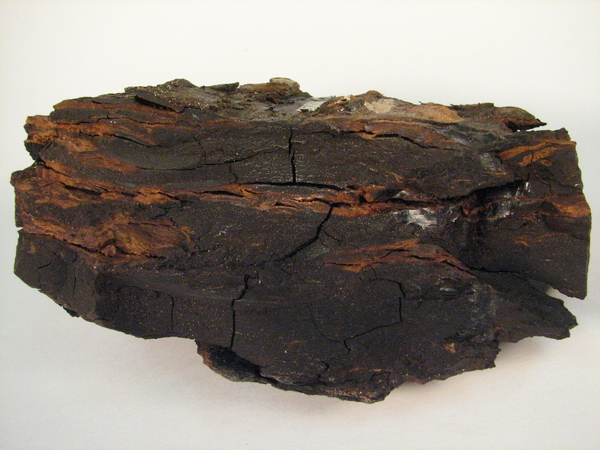
\includegraphics[width=\textwidth]{lignit}
			\begin{itemize}
				\item najmenej kvalitný typ
				\item najmladšie
				\item najviac znečistujúce
			\end{itemize}
		\end{column}
		\begin{column}{.48\textwidth}
			Čierne uhlie - Antracit
			\begin{itemize}
				\item najviac kvalitný typ
				\item najstaršie
				\item najmenej znečistujúce
			\end{itemize}
			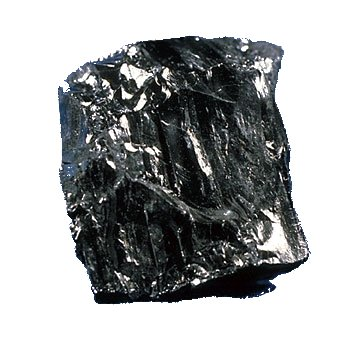
\includegraphics[width=\textwidth]{antracit}
		\end{column}
	\end{columns}
\end{frame}

\section{Ťažba}

\renewcommand{\arraystretch}{1.5}

\begin{frame}
	\frametitle{Ťažba uhlia vo svete}
	\centering

	\only<1>{
	Množstvo vyťaženého uhlia podľa krajiny milíonoch ton uhlia za rok 2021\\[1.5em]
	\begin{tabular}{ |c|c| }
		\hline
		Čína & 4126\\
		\hline
		India & 762\\ 
		\hline
		Indonézia & 614\\
		\hline
		Spojené štáty americké & 523\\
		\hline
		Austrália & 467\\
		\hline
		Rusko & 435\\
		\hline
		Južná Afrika & 235\\
		\hline
	\end{tabular}
	}

	\only<2>{
		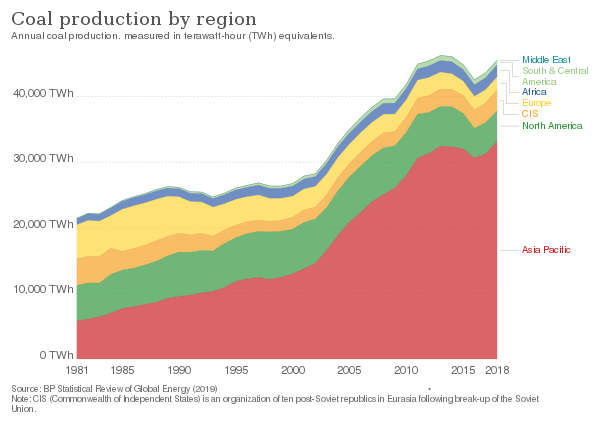
\includegraphics[width=\textwidth]{tazba-graf}
	}
\end{frame}

\begin{frame}
	\Large
	\centering

	\only<1>{
	Austrália\\[1em]
	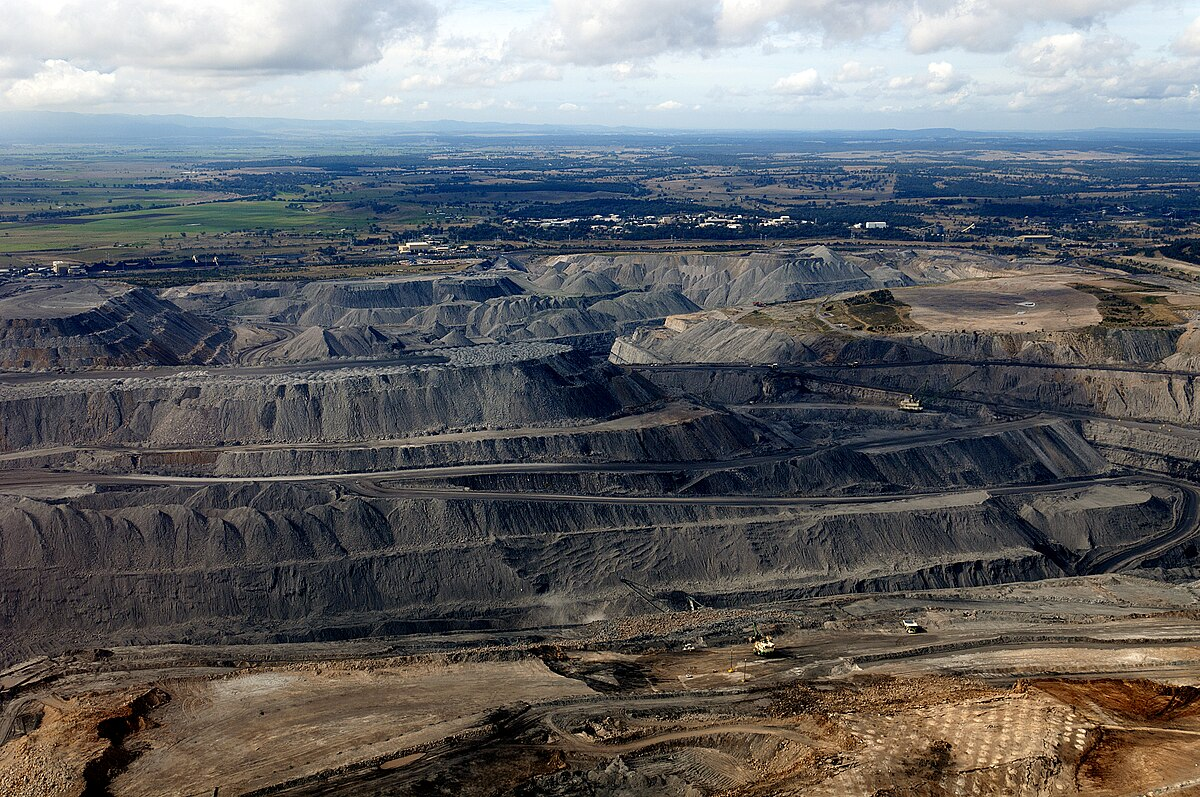
\includegraphics[width=\textwidth]{australia-tazba}
	}
	\only<2>{
	Nemecko\\[1em]
	\includegraphics[width=\textwidth]{nemecko-tazba}
	}
	\only<3>{
	Čína\\[1em]
	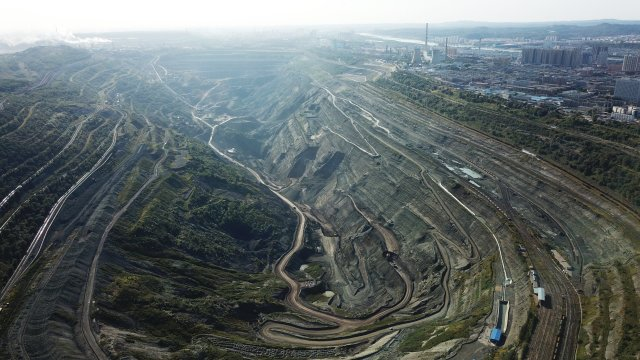
\includegraphics[width=\textwidth]{tazba-china}
	}
\end{frame}

\begin{frame}
	Danke za pozornosť

	\pause

	\begin{itemize}
		\item \url{https://referaty.aktuality.sk/vznik-uhlia/referat-17235}
		\item \url{https://www.uhlie.com/informacie/28-vseobecne-informacie-o-uhli}
		\item \url{https://en.wikipedia.org/wiki/List_of_countries_by_coal_production}
		\item \url{https://www.wsj.com/articles/the-real-war-on-coal-is-in-china-1510644712}
	\end{itemize}
\end{frame}
\end{document}
